\section{Results}
Next we evaluate the sparsemax transformation on a series of benchmark datasets using our four different implementations. We use a  model equivalent to a logistic regression, but where the activation function at the output layer is sparsemax rather than softmax. For comparison we report the softmax results as well. Our four different implementations are refered to in the following as follows:
\begin{itemize}
\item Softmax: A TensorFlow implementation of Softmax Regression
\item Numpy: A Numpy implementation of Sparsemax Regression
\item TF Numpy: A TensorFlow implementation where the custom ops associated with Sparsemax have been implemented using only Numpy
\item TF CPU: A TensorFlow implementation where the custom ops associated with Sparsemax have been implemented in C++. This version runs only at the CPU.
\item TF GPU: A TensorFlow implementation where the custom ops associated with Sparsemax have been implemented in C++. This version runs only at the CPU.
\end{itemize}
For the sake of timing comparison we will compare all five implementations, while for the performance only the TensorFlow CPU version of Sparsemax will be compared with the Softmax implementation as the results are equivalent for all Sparsemax implementations as expected.
\subsection{Label estimation}
We use five well-known benchmark datasets shown in Table \ref{tab:datasets}. The digit dataset MNIST and flower dataset Iris are multi-class classification, while the Scene, Emotions and CAL500 datasets are multi-label classification. \footnote{In multi-class classification the classes are mutually exclusive, while in the multi-label case several labels can be associated with one observation reflecting a relation between the labels.} We report the Jensen-Shannon divergence betweent the predicted and target distributions:
\begin{equation}
\mathbf{JS(q,p)}:=\frac{1}{2}\mathbf{KL}(\mathbf{q}||\frac{\mathbf{q}+\mathbf{p}}{2})+\frac{1}{2}\mathbf{KL}(\mathbf{p}||\frac{\mathbf{q}+\mathbf{p}}{2})
\end{equation}
Where $\mathbf{p}, \mathbf{q}$ are the predicted and target distributions, respectively and $\mathbf{KL}$ the Kullbach-leibler distance. For all the classifiers we use a L2 regualizer where the regualization constant used can be seen in Table \ref{tab:hyperparameters}. These have been chosen using cross-validation, where the resulting experiments are shown in Figure \ref{fig:hyperparameters}.

\begin{table}[H]
\centering
\begin{tabular}{r|cccc}
& \#Features & \#Labels & Train size & Test size \\
\hline
MNIST & 784 & 10 & 60000 & 10000 \\
Iris & 4 & 3 & 135 & 15 \\
Scene & 294 & 6 & 1211 & 1196 \\
Emotions & 72 & 6 & 391 & 202 \\
CAL500 & 68 & 174 & 451 & 51 \\
\end{tabular}

\caption{Statistics for the five benchmark datasets used.}
\label{tab:datasets}
\end{table}


\begin{table}[H]
\centering
\begin{tabular}{r|ccc}
& Softmax & Sparsemax \\
\hline
MNIST & $1.00 \cdot 10^{-7}$ & $1.00 \cdot 10^{-6}$ \\
Iris & $1.00 \cdot 10^{-8}$ & $1.00 \cdot 10^{-8}$ \\
Scene & $1.00 \cdot 10^{-8}$ & $1.00 \cdot 10^{-4}$ \\
Emotions & $1.00 \cdot 10^{-8}$ & $1.00 \cdot 10^{-2}$ \\
CAL500 & $1.00 \cdot 10^{-8}$ & $1.00 \cdot 10^{-1}$ \\
\end{tabular}

\caption{Values for the regualizers used in both classifiers.}
\label{tab:hyperparameters}
\end{table}

\begin{figure}[H]
	\centering
	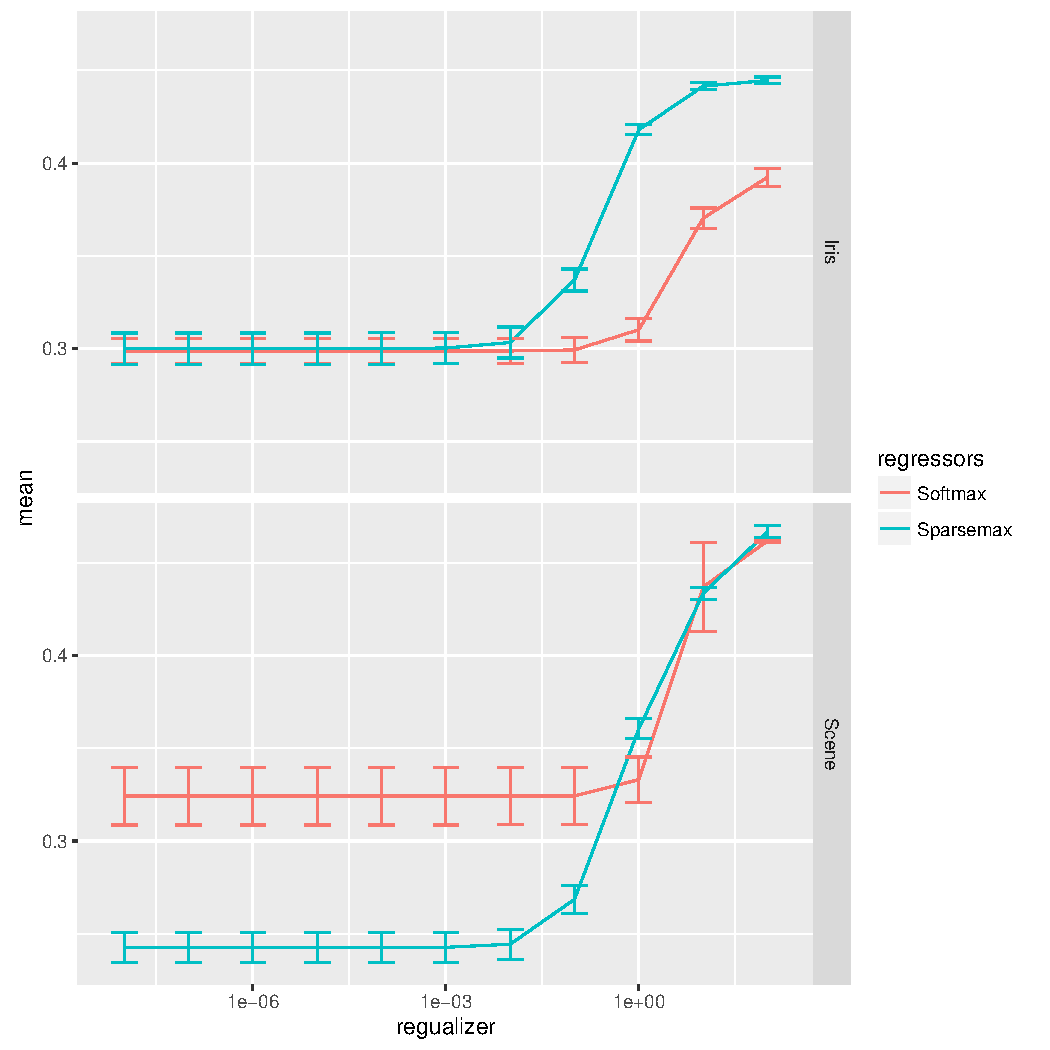
\includegraphics[width=\columnwidth]{figures/hyperparameter.pdf}
\caption{JS divergence using a range of regualizers on all five datasets for the two regressors.}
\label{fig:hyperparameters}.
\end{figure}

\begin{table}[H]
\centering
\begin{tabular}{r|ccc}
& Softmax & Sparsemax \\
\hline
MNIST & $inf \pm nan$ & $0.10 \pm 0.00$ \\
Iris & $0.15 \pm 0.00$ & $0.10 \pm 0.01$ \\
Scene & $0.30 \pm 0.01$ & $0.24 \pm 0.01$ \\
Emotions & $0.29 \pm 0.02$ & $0.27 \pm 0.02$ \\
CAL500 & $0.35 \pm 0.01$ & $0.35 \pm 0.01$ \\
\end{tabular}

\caption{$\mathbf{JS}$ divergence for the five benchmark datasets and the Sparsemax Classifier as well as the Softmax classifier.}
\end{table}


\begin{table*}
\centering
\begin{tabular}{r|ccc}
& digits & iris \\
\hline
sparsemax - tensorflow numpy & $0.02 \pm 0.00$ & $0.00 \pm 0.00$ \\
sparsemax - tensorflow native & $0.01 \pm 0.00$ & $0.00 \pm 0.00$ \\
sparsemax - numpy & $0.01 \pm 0.00$ & $0.00 \pm 0.00$ \\
softmax - tensorflow & $0.02 \pm 0.00$ & $0.00 \pm 0.00$ \\
\end{tabular}

\caption{Relative time with associated confidence intervals.}
\end{table*}





